\documentclass[utf8,10pt]{beamer}
\usepackage{fontspec,xeCJK,booktabs,array,tabularx,listings}
\usepackage{geometry,amsmath,amssymb,theorem,caption,extarrows,mathrsfs,bm}
\usepackage{graphicx,xcolor,listings,geometry,booktabs,tikz}
\usepackage{pgfplots,grffile}
\pgfplotsset{compat=newest}
  %% the following commands are needed for some matlab2tikz features
\usetikzlibrary{plotmarks}
\usetikzlibrary{arrows.meta}
\usetikzlibrary{calc}
\usepgfplotslibrary{patchplots}
\setmainfont{CMU Serif}
\setsansfont{CMU Sans Serif}
\setmonofont{Sarasa Mono SC Nerd}
\setCJKmainfont{FandolSong}
\setCJKsansfont{FandolSong}
\setCJKfamilyfont{song}{FandolSong}
\newcommand{\song}{\CJKfamily{song}}
\setCJKfamilyfont{kaiti}{FandolKai}
\newcommand{\kaiti}{\CJKfamily{kaiti}}
\setCJKfamilyfont{heiti}{FandolHei}
\newcommand{\heiti}{\CJKfamily{heiti}}
\definecolor{GreenDarkFaded}{rgb}{0,0.6,0}
\definecolor{SpringGreenDark}{rgb}{0.2,0.6,0}
\definecolor{GreenObscureWeak}{rgb}{0,0.2,0}
\definecolor{GreenDarkDull}{rgb}{0.2,0.6,0.2}
\lstdefinestyle{lfonts}{
  basicstyle   = \scriptsize\ttfamily,
  stringstyle  = \color{purple},
  keywordstyle = \color{blue!60!black}\bfseries,
  commentstyle = \color{olive}\scshape,
}
\lstdefinestyle{lnumbers}{
  numbers     = left,
  numberstyle = \tiny,
  numbersep   = 1em,
  firstnumber = 1,
  stepnumber  = 1,
}
\lstdefinestyle{llayout}{
  breaklines       = true,
  tabsize          = 2,
  columns          = spacefixed,
  showstringspaces = false,
  showtabs         = false,
}
\lstdefinestyle{lgeometry}{
  xleftmargin      = 20pt,
  xrightmargin     = 0pt,
  frame            = tb,
  framesep         = \fboxsep,
  framexleftmargin = 20pt,
}
\lstdefinestyle{lgeneral}{
  style = lfonts,
  style = lnumbers,
  style = llayout,
  style = lgeometry,
}
\mode<presentation>
{
 \usetheme{Berkeley}
 \usecolortheme{spruce}
 \usecolortheme[named=GreenDarkDull]{structure}
 \setbeamercovered{transparent}
}
\usepackage{pdfpages}
\usepackage{navigator}
\usepackage{subfig}
\usepackage{graphics,tcolorbox,hyperref}


\title{MATLAB编程实现电子乐合成器}
\author{仇琨元 11913019}
\date{\footnotesize \vspace{5mm}\today}


\begin{document}
\begin{frame}

    \titlepage

\end{frame}
\begin{frame}
    \frametitle{TOC}

    \tableofcontents

\end{frame}

\section{Introduction}
\begin{frame}
    \frametitle{电子乐简介}

    \begin{itemize}
        \item 音乐是组织特定时域波形的声音信号的艺术形式。
        \item DSP技术可以依据人的主观意愿任意生成声音信号。
    \end{itemize}

    \textbf{电子音乐}是一种使用数字信号处理技术合成音乐声音信号的音乐艺术。

    \begin{figure}[htpb]
        \centering
        \subfloat[合成器的一部分子程序代码]{
            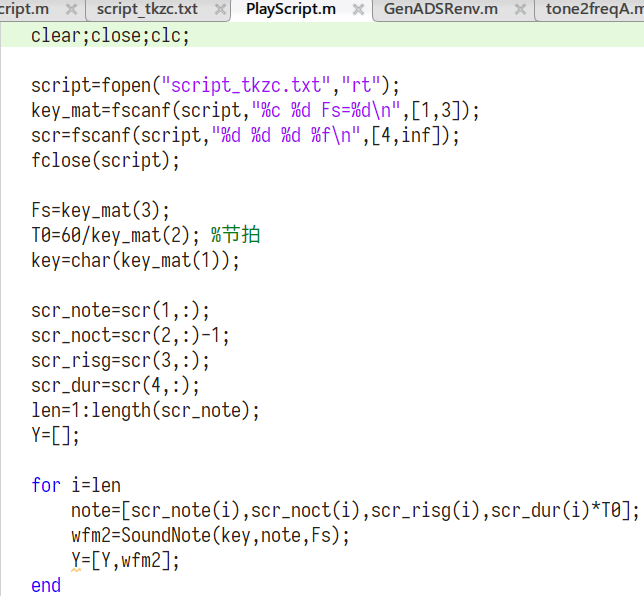
\includegraphics[height=0.5\textheight]{figures/demo_fig.png}
        }\hfill
        \subfloat[VOCALOID(一种人声合成器)的编辑界面]{
            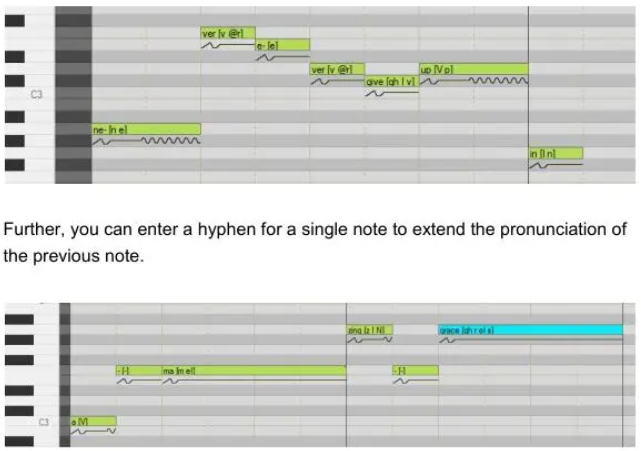
\includegraphics[width=0.45\textwidth]{figures/20221116104915.png}
        }
        \caption{电子乐合成器}
        \label{fig:synthesizer}
    \end{figure}

\end{frame}

\begin{frame}
    \frametitle{项目简介}

    本项目使用 MATLAB 编程环境实现简单的包络合成器合成电子音乐。该合成器具有以下能力:

    \begin{itemize}
        \item 从文件读取简单的乐谱,包含音符、调号和节拍信息。
        \item 基于乐器振动方程和实测频谱数据生成连续单音。
        \item 基于实际乐器共振腔体频率响应的频域滤波处理(音色生成器)。
        \item 可任意调节参数的 ADSR 包络发生器。
    \end{itemize}

    \begin{figure}[htpb]
        \centering
        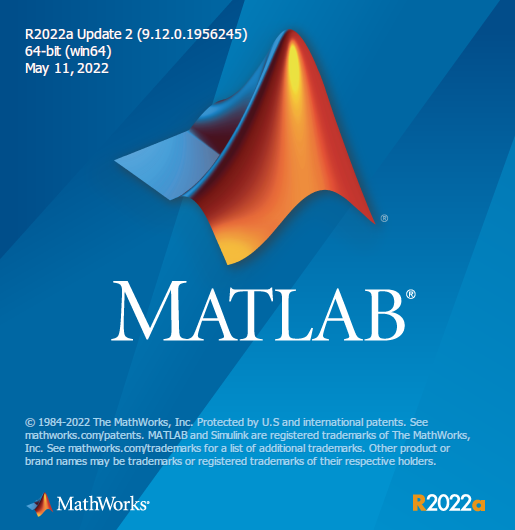
\includegraphics[height=0.4\textheight]{figures/20221116102905.png}
        \label{fig:matlab}
    \end{figure}

\end{frame}

\section{合成器总体架构}
\begin{frame}
    \frametitle{合成器结构框图}

    \begin{figure}[htpb]
        \centering
        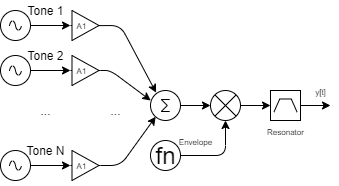
\includegraphics[height=0.5\textheight]{figures/synth_arch.png}
        \caption{合成器总体架构}
        \label{fig:synthesizer_arch}
    \end{figure}

    合成器首先通过傅里叶逆变换生成具有乐器 STFT (短时傅里叶变换)频谱的连续波,然后用音色滤波器进行进一步的频域处理,从而获得具有\textbf{一部分音色}的连续波乐音信号。

    将连续波信号乘上一定的 ADSR 包络线,即可产生具有完整音色的时域波形。

\end{frame}

\begin{frame}
    \frametitle{合成器结构框图}

    为了方便用户使用,合成器只需要读取特定格式的乐谱文件即可演奏音乐,乐谱文件不应固化到前述的数字信号处理模块内部。

    由此可见,合成器应当具有如下组成部分:

    \begin{itemize}
        \item 乐谱读取
        \item 调号、音符到频率数值计算
        \item 连续波合成器
        \item 音色滤波器
        \item 包络发生器
    \end{itemize}

\end{frame}

\section{音阶发生器}
\subsection{人耳频率响应}
\begin{frame}
    \frametitle{人耳频率响应与音阶划分}

    人类听觉系统通过耳蜗对声音信号进行频谱分解。耳蜗基底膜受到声音信号刺激后会发生响应,产生振动。

    基底膜的宽度和厚度随着耳蜗螺距逐渐变化,研究表明基底膜顶部到谐振点的直线距离与输入频率的对数成正比,因此人耳在频谱上有近似对数标度的响应。

    \begin{figure}[htpb]
        \centering
        \subfloat[耳蜗结构简图]{
            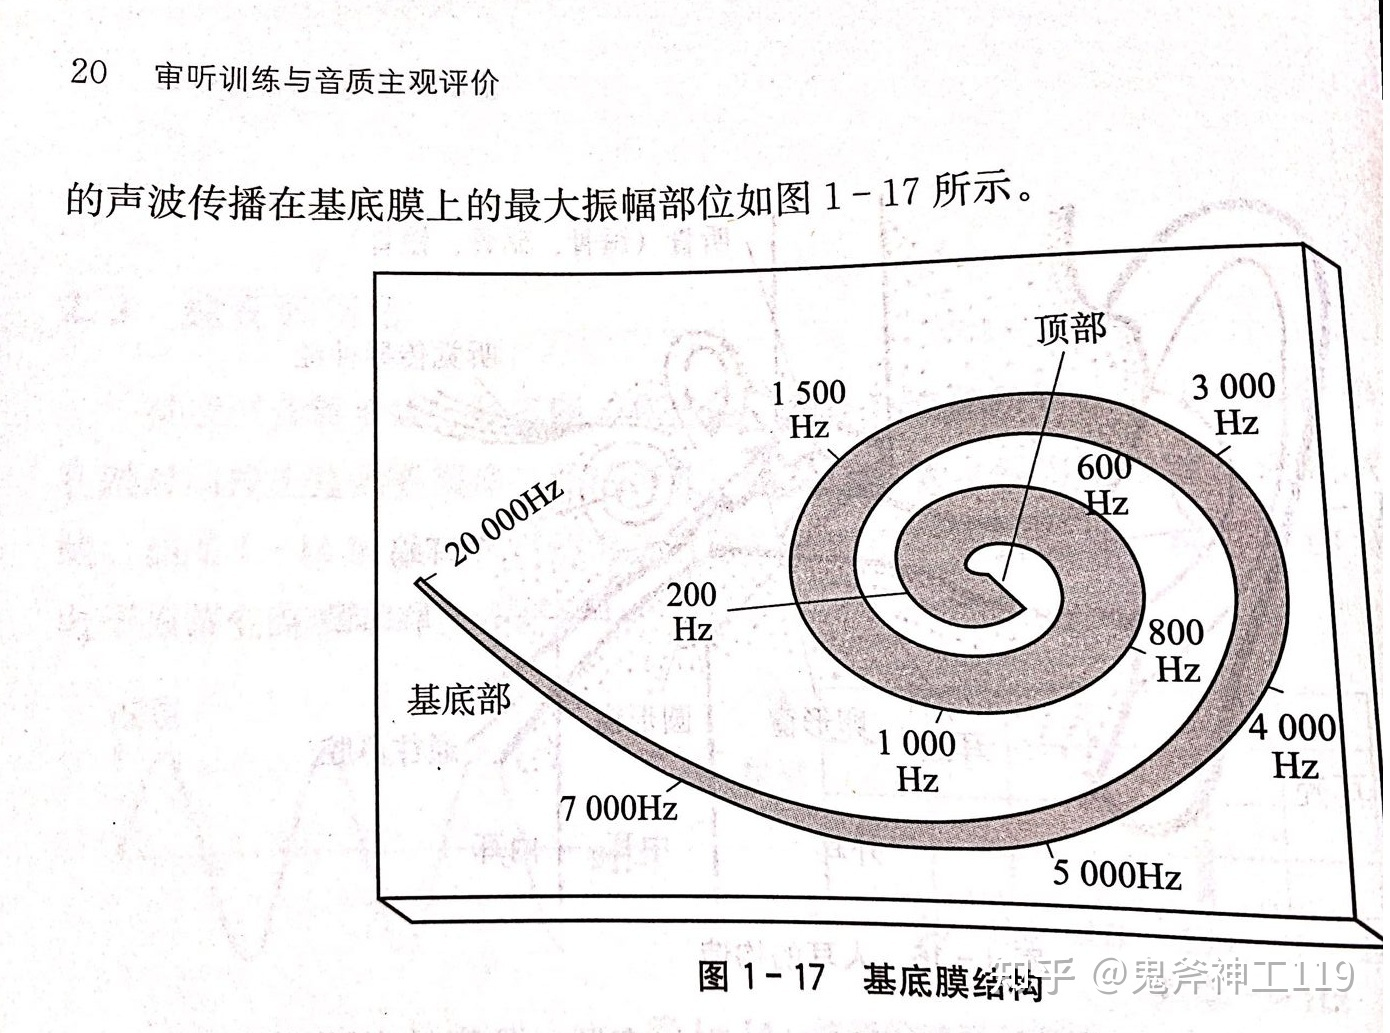
\includegraphics[height=0.4\textheight]{figures/20221117105915.png}
        }\hfill
        \subfloat[人类听觉等响度曲线]{
            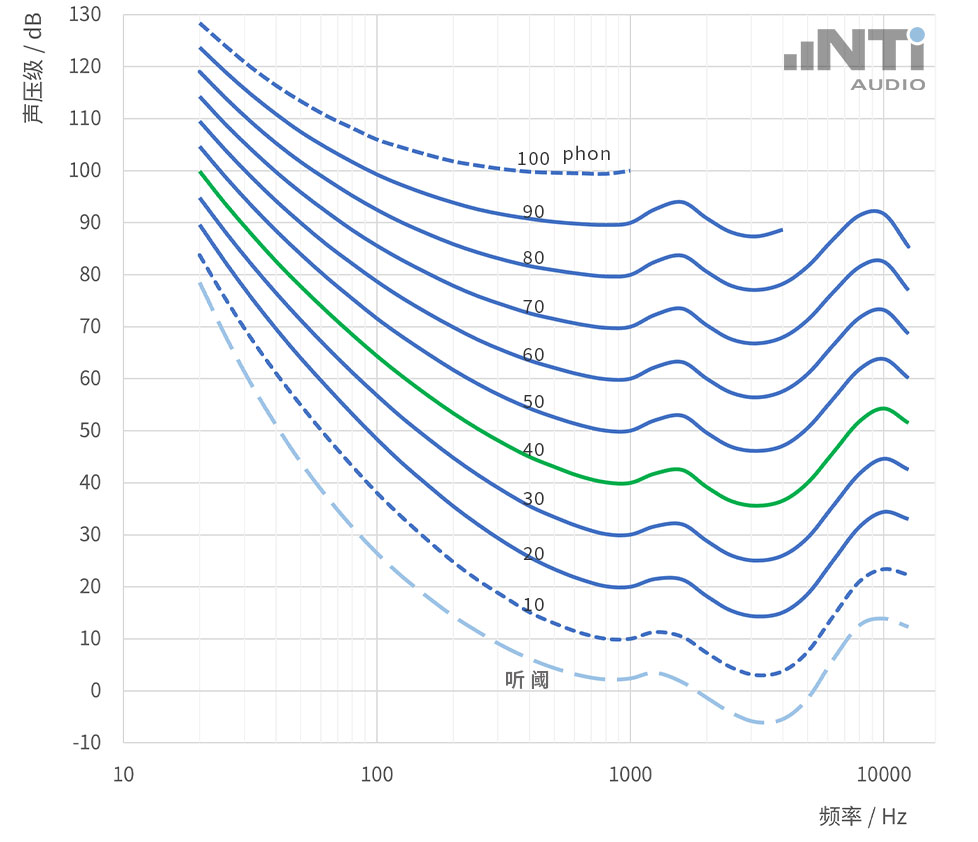
\includegraphics[height=0.4\textheight]{figures/20221117110049.png}
        }
        \caption{人类听觉系统简图}
        \label{fig:acoustic_system}
    \end{figure}

\end{frame}

\begin{frame}
    \frametitle{人耳听觉音域}

    长期的归纳总结和前述\textbf{对数标度律}均指出,绝对频率为整数倍的纯音(复指数信号\(Ae^{j\omega t}\))在听觉感知中表现为线性的整数音高差,而两个音的绝对频率比越接近1:1,混频后的和声就越和谐。

    这种整数音高差的最小单位为一个倍频程\(\Delta f=f_0\),称为一个\textbf{八度}。以人耳最敏感的中音\(A_0=440\text{Hz}\)作为标定原点,人耳听觉范围大约能覆盖

    \begin{equation}
        \left\lceil \frac{\log(\frac{f_{min}}{440})}{\log(2)} \right\rceil=-4, \left\lfloor \frac{\log(\frac{f_{max}}{440})}{\log(2)} \right\rfloor=5
    \end{equation}

    共计9个八度。

\end{frame}

\subsection{十二平均律}
\begin{frame}
    \frametitle{十二平均律}

    在一个八度之内选取人耳最敏感的7个相对音高频点,这些频点的频率均近似处于一个首项等于公比的等比数列上。

    \begin{figure}[htpb]
        \centering
        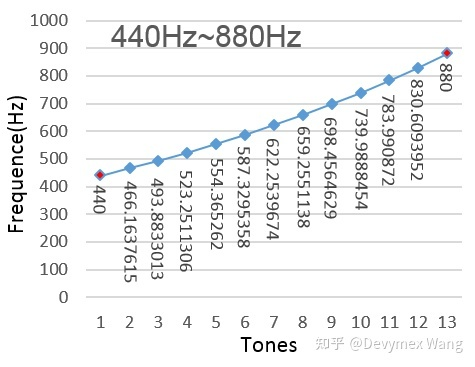
\includegraphics[height=0.4\textheight]{figures/20221117120845.png}
    \end{figure}

    一般来说这7个谐频点含有2个倍频程为\(q\)的频点和5个倍频程为\(q^{2}\)的频点。由此可得一个八度内7个相对音高频点的分布律
    \begin{equation}
        q^{2}\cdot (q^{2})^{5}=2\Rightarrow q=2^{\frac{1}{12}}\approx 1.06
    \end{equation}

\end{frame}

\begin{frame}
    \frametitle{十二平均律}

    因此,一个八度之内的12个半音频点即可用上述的公比计算:
    \begin{equation}
        f[k]=f_0 q^{k}=f_0 2^{\frac{k}{12}}
    \end{equation}
    在文艺复兴时期以来的实际音乐创作中,一般以\(C_1=523\text{Hz}\)标定八度音阶起始点,因而包含2个半音和5个全音的音阶序列
    \begin{equation}
        k=[0,2,4,5,7,9,11]
    \end{equation}
    被称为大调音阶。将前述的八度音程规约(1)代入(3),即可得到用十二平均律系统表示的任意音高记号到频率的转换公式:

    \begin{equation}
        f[k]=f_{C1}2^{(k_{0}+k)/12+p},p\in[-4,5],\{k_{0},k\}\subset\{0,2,4,5,7,9,11\}
    \end{equation}

\end{frame}

\subsection{代码实现}
\begin{frame}[fragile]
    \frametitle{音符到音阶转换代码}

    \begin{lstlisting}[language=matlab,style=lgeneral,gobble=3]
    function freq=tone2freq(tone,noctave,rising,base,minority)
        if tone<1||tone>7
            error("输入的音符 %d 不在表示范围 [1,7] 内",tone);
        end
        tbl1=ToScale(base,minority);
        freq=440*2.^((tbl1(tone)+rising)/12+noctave);
    end
    function table=ToScale(Base,Minority)
        scale1=cumsum([2,1,2,2,1,2,2]);
        scale2=cumsum([2,2,1,2,2,2,1]);
        if all(isa(Base,'char'))
            Base=Base-'A';
        end
        minor=[4,3,3,4,4,3,4];
        if Base==0
            table=[0,scale2]-(Minority~=0)*4;
        else
            table=scale1(Base)+[0,scale2]-(Minority~=0)*minor(Base);
        end
    end
    \end{lstlisting}

\end{frame}

\section{连续波合成器}

\subsection{钢琴弦振动方程}
\begin{frame}
    \frametitle{钢琴弦振动方程}

    合成器依据钢琴弦振动方程和实测频谱数据产生具有钢琴音色的单音。钢琴弦的振动可以用一维弦振动模型描述:
    \begin{equation}
        \begin{cases}
            u_{tt}+\mu u_{t}  & =v^{2}u_{xx},                                                                               \\
            u|_{x=0}=u|_{x=l} & =0,                                                                                         \\
            u|_{t=0}          & =0,                                                                                         \\
            u_{t}|_{t=0}      & =\text{rect}\left( \frac{x-x_{0}}{2d} \right)v_{0}\cos\left( \pi \frac{x-x_{0}}{2d} \right)
        \end{cases}
    \end{equation}

    时域波形遵循该亥姆霍兹方程的解:
    \begin{equation}
        \begin{cases}
            u(x,t)   & =A\exp(-\mu/2 t) \sum_{n=1}^{\infty} \frac{1}{n}\frac{1}{1-4d^2n^2/l^2}B(n,x,t), \\
            B(n,x,t) & =C_{n}\sin(n\pi x_{0}/l)sin(n\omega_0 t)                                         \\
                     & +D_{n}\cos(n\pi x_{0}/l)\cos(n\omega_0 t)
        \end{cases}
    \end{equation}

\end{frame}

\begin{frame}
    \frametitle{钢琴弦振动方程}

    由于解析解的两个傅里叶系数\(C_n,D_n\)难以求解,因此用实际测量的频谱数据代替根据琴弦物理参数解析求解。根据现有研究,利用以下经验公式确定谐波最高阶数:

    \begin{equation}
        N_{max}=\left\lceil \frac{f_{A1}\times N_{A1}}{f[k]} \right\rceil
    \end{equation}

    其中\(N_{A1}\)是对最终合成音色有可辨识影响的最高谐波阶数:
    \begin{equation}
        \frac{B^{2}[N_{A1}]+C^{2}[N_{A1}]}{\sum(B_{n}^{2}+C_{n}^{2})}\lvert_{440\text{Hz}}>30\text{dB}
    \end{equation}

\end{frame}

\subsection{代码实现}
\begin{frame}[fragile]
    \frametitle{代码实现}

    \begin{lstlisting}[language=matlab,style=lgeneral,gobble=4]
    function wfm2=SoundNote(key,note,Fs)
        duration=note(4);
        Tv=linspace(0,duration,duration*Fs);
        if note(1)==0
            wfm2=zeros(1,round(duration*Fs));
        else
            fc1=tone2freq(note(1),note(2),note(3),key,0);
            fc1_list=fc1*(1:19);
            amp=[987.8,368.6,620.2,483.9,156.7,83.62,120.1, ...
                 70.73,5.348,24.41,27.35,21.3,10.31,6.477, ...
                 15.91,3.495,2.546,0.4751,0.8858]/1000;
            wfm1=cell2mat(arrayfun(@(a,x) a*sin(2*pi*x*Tv),amp,fc1_list,'UniformOutput',false).');
            wfm1=sum(wfm1,1).*GenADSRenv(wfm1,[0.008,0.09,0.11,0.25,0.67],[0.88,0.88,0.56,0.50,0]);
            [b_b1,a_b1]=butter(6,2*[1300,1900]/Fs);
            [b_b2,a_b2]=butter(6,2*[3600,5000]/Fs);
            [b_b3,a_b3]=butter(6,2*[7800,8200]/Fs);
            wfm2=1.1*wfm1+0.4*filter(b_b1,a_b1,wfm1)+0.35*filter(b_b2,a_b2,wfm1)+0.25*filter(b_b3,a_b3,wfm1);
            wfm2=wfm2/(max(wfm2));
        end
    end
    \end{lstlisting}

\end{frame}

\section{包络发生器}

\subsection{ADSR 包络}
\begin{frame}
    \frametitle{ADSR 包络}

    声音的时间包络(Time Envelope)也是音色的一个重要组成部分。相同的频谱,在不同的时间包络下,会让我们听到截然不同的声音。电子乐领域一般用 ADSR 模型(\ref{fig:adsr_concept})构造包络。

    \begin{figure}[htpb]
        \centering
        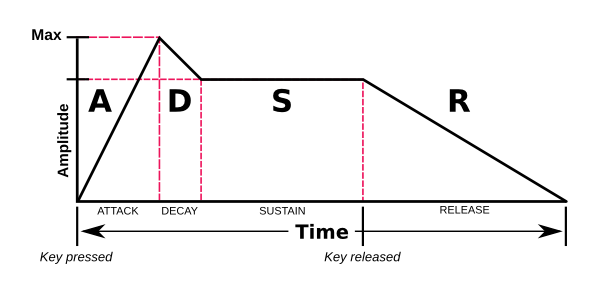
\includegraphics[height=0.4\textheight]{figures/adsr_concep.png}
        \caption{ADSR 的概念}
        \label{fig:adsr_concept}
    \end{figure}

    声音从无到有,从有到无,都需要经历一个过渡变化的阶段,我们将声音从无到有的这段时间,叫做上升时间(Attack Time),而将声音从有到无的时间,叫做释放时间(Release Time)。

\end{frame}

\begin{frame}
    \frametitle{钢琴的 ADSR 特征}

    像钢琴这样的乐器,除了按下琴键时上升时间很短之外,琴弦在按下琴键后到抬起手指之前还会持续振动,因而钢琴会持续发声。

    \begin{figure}[htpb]
        \centering
        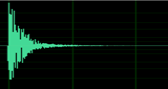
\includegraphics[height=0.4\textheight]{figures/adsr_real_piano.png}
        \caption{实际测量的钢琴音符波形}
        \label{fig:real_piano_adsr}
    \end{figure}

    在这段时间里,琴弦的振动会随着时间缓慢减弱。这段振幅慢慢减小的时间叫做衰减时间(Decay Time)。

\end{frame}

\subsection{代码实现}
\begin{frame}[fragile]
    \frametitle{折线 ADSR 包络的代码实现}

    使用两点式方程和阶跃函数实现(\ref{fig:adsr_concept})中的折线 ADSR 包络。

    \begin{lstlisting}[language=matlab,style=lgeneral,gobble=4]
    function env=GenADSRenv(x,vx,vy)
        tv=linspace(0,1,length(x));
        vxi=[0,vx];
        vyi=[0,vy];
        ya=zeros(1,length(tv));
        for i=1:(length(vxi)-1)
            ya=ya+Line(tv,[vxi(i),vyi(i)],[vxi(i+1),vyi(i+1)]).*(tv>=vxi(i)&tv<vxi(i+1));
        end
        env=ya;
    end
    function y=Line(x,p1,p2)
        y=(x-p2(1)).*(p2(2)-p1(2))./(p2(1)-p1(1))+p2(2);
    end
    \end{lstlisting}

\end{frame}

\section{乐谱文件读取}

\subsection{代码实现}
\begin{frame}
    \frametitle{乐谱文件结构}

    \begin{figure}[htpb]
        \centering
        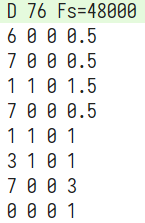
\includegraphics[height=0.6\textheight]{figures/20221117132924.png}
    \end{figure}

    乐谱文件由包含调号、节拍和抽样率的文件头与音符表组成。

\end{frame}

\begin{frame}[fragile]
    \frametitle{文件读取模块}

    \begin{lstlisting}[language=matlab,style=lgeneral,gobble=4]
        script=fopen("script_collective.txt","rt");
        key_mat=fscanf(script,"%c %d Fs=%d\n",[1,3]);
        scr=fscanf(script,"%d %d %d %f\n",[4,inf]);
        fclose(script);

        Fs=key_mat(3);
        T0=60/key_mat(2); %节拍
        key=char(key_mat(1));

        scr_note=scr(1,:);
        scr_noct=scr(2,:)-1;
        scr_risg=scr(3,:);
        scr_dur=scr(4,:);
        len=1:length(scr_note);
        Y=[];

        for i=len
            note=[scr_note(i),scr_noct(i),scr_risg(i),scr_dur(i)*T0];
            wfm2=SoundNote(key,note,Fs);
            Y=[Y,wfm2];
        end
    \end{lstlisting}

\end{frame}

\end{document}